\section{Istruzioni per l'uso}
\subsection{Requisiti di sistema}
Descrizione di tutti i requisiti necessari a funzionamento dell'applicazione Premi.

\subsection{Guida all'installazione???}
Serve? Boh...

\subsection{Primo accesso}
Al primo accesso il sistema richiede l'autenticazione dell'utente qualora fosse già registrato al sistema, altrimenti fornisce la possibilità di creare un nuovo account.
\begin{figure}[h]
\begin{center}
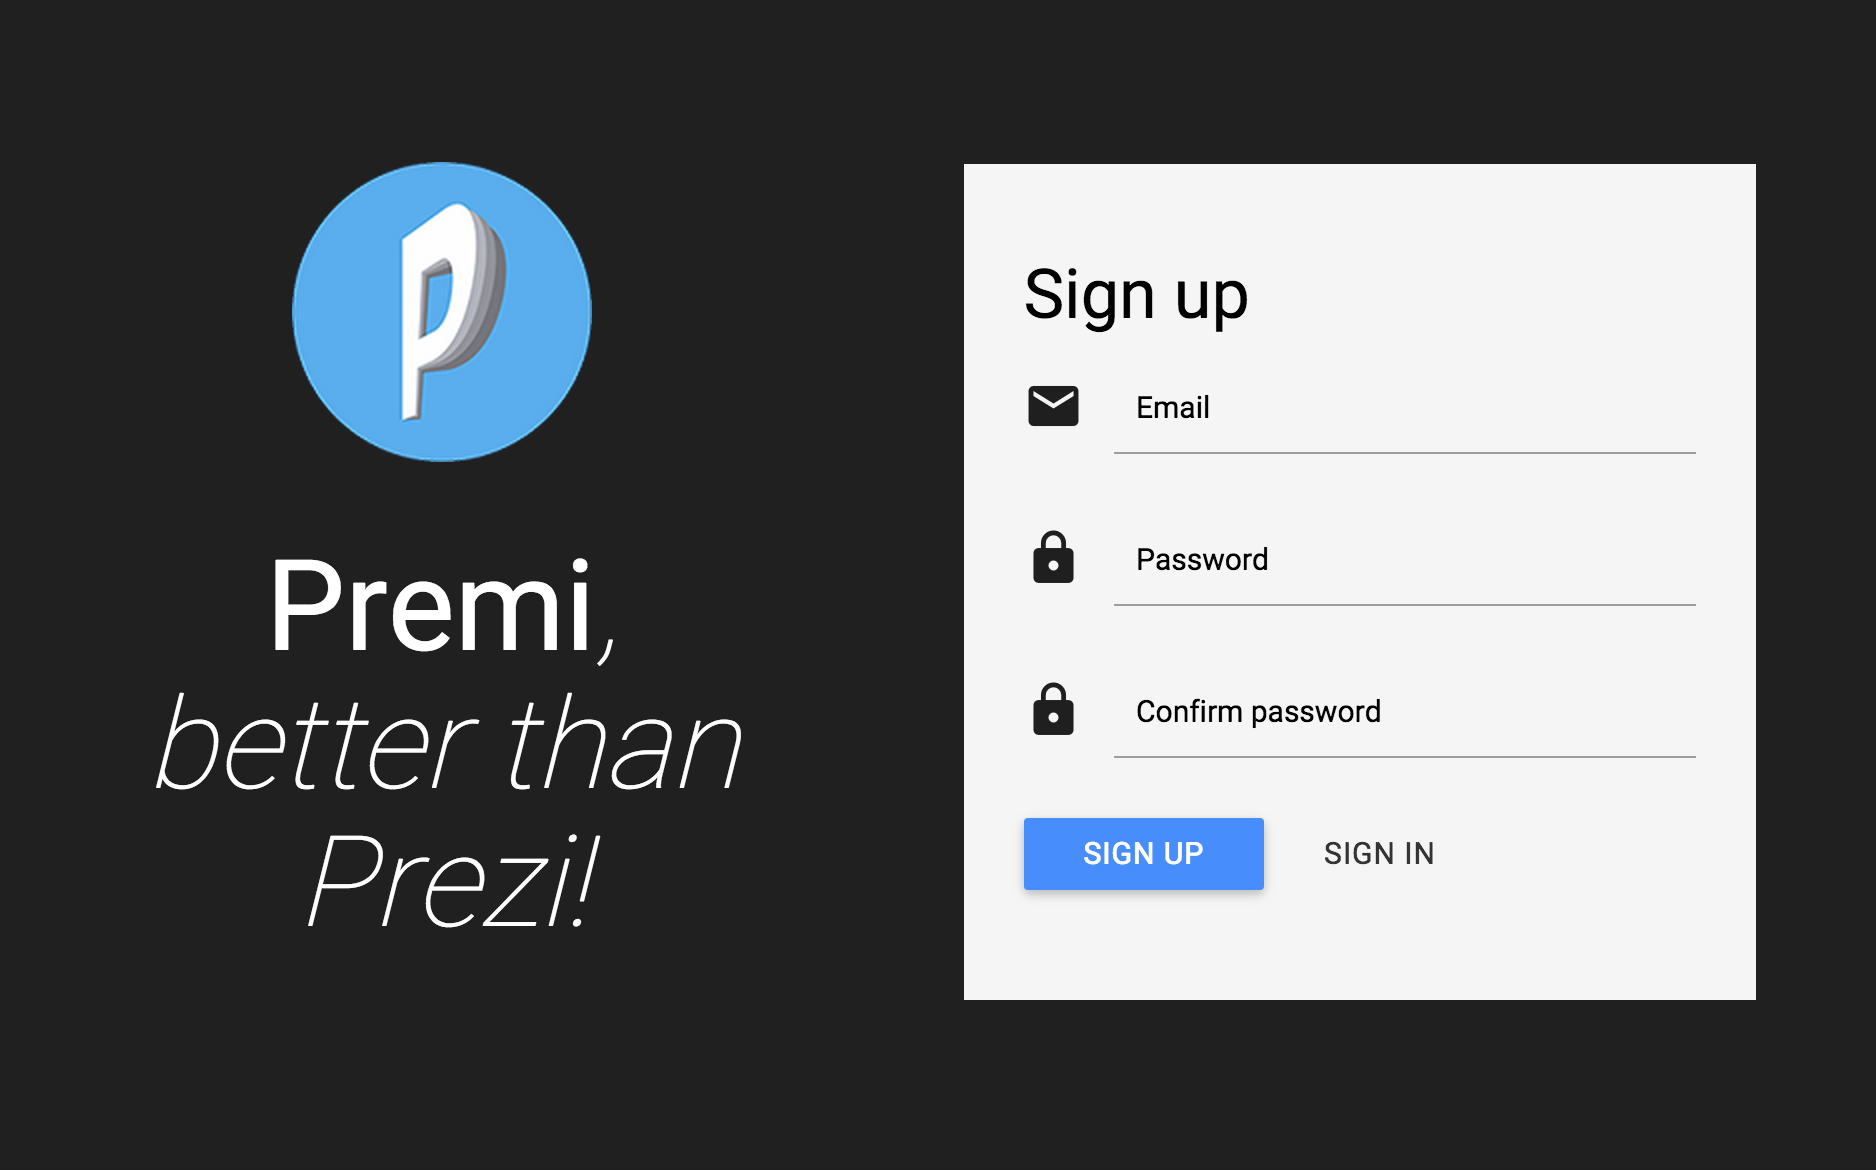
\includegraphics[scale=0.4]{img/signup.png}
\caption{Form di registrazione.}
\end{center}
\end{figure}

Per la creazione di un nuovo account i dati da inserire sono soggetti ad alcuni vincoli:
\begin{itemize}
\item Indirizzo email: deve essere un indirizzo valido;
\item Password: composta da almeno n. caratteri;
\item Conferma password: deve coincidere con il campo password precedente.
\end{itemize}
Per confermare la registrazione premere sul tasto "SIGN UP".
\begin{quote}
\textbf{Nota:} si potrebbero ricevere degli avvisi che notificano l'errato inserimento dei dati richiesti.
\end{quote}
Una volta completata la registrazione è necessario autenticarsi al sistema:
\begin{figure}[h]
\begin{center}
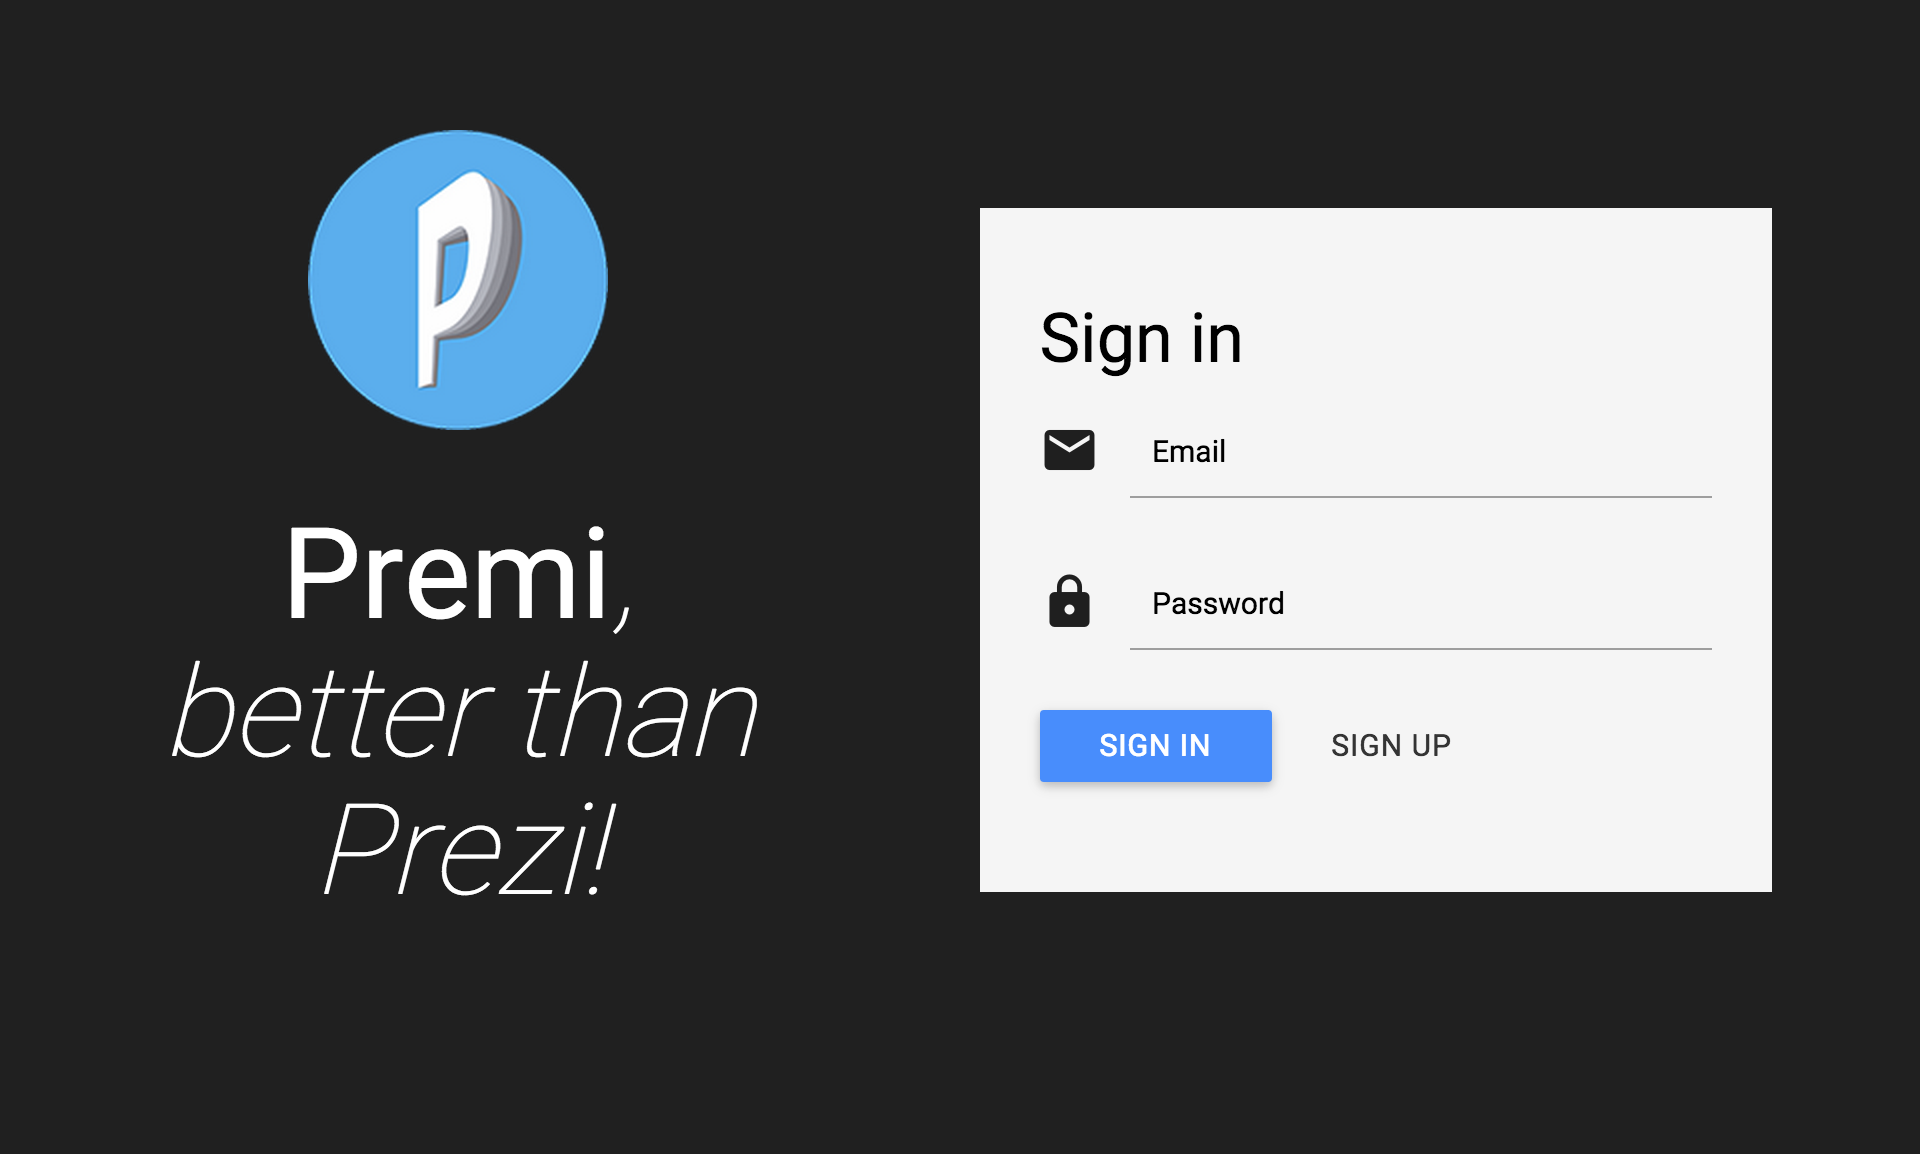
\includegraphics[scale=0.4]{img/signin.png}
\caption{Autenticazione al sistema.}
\end{center}
\end{figure}

\newpage
\subsection{Pannello di controllo dell'utente}
Una volta autenticati al sistema si accede al proprio pannello di controllo, all'interno del quale saranno visibili tutte le presentazioni finora create.
\begin{figure}[h]
\begin{center}
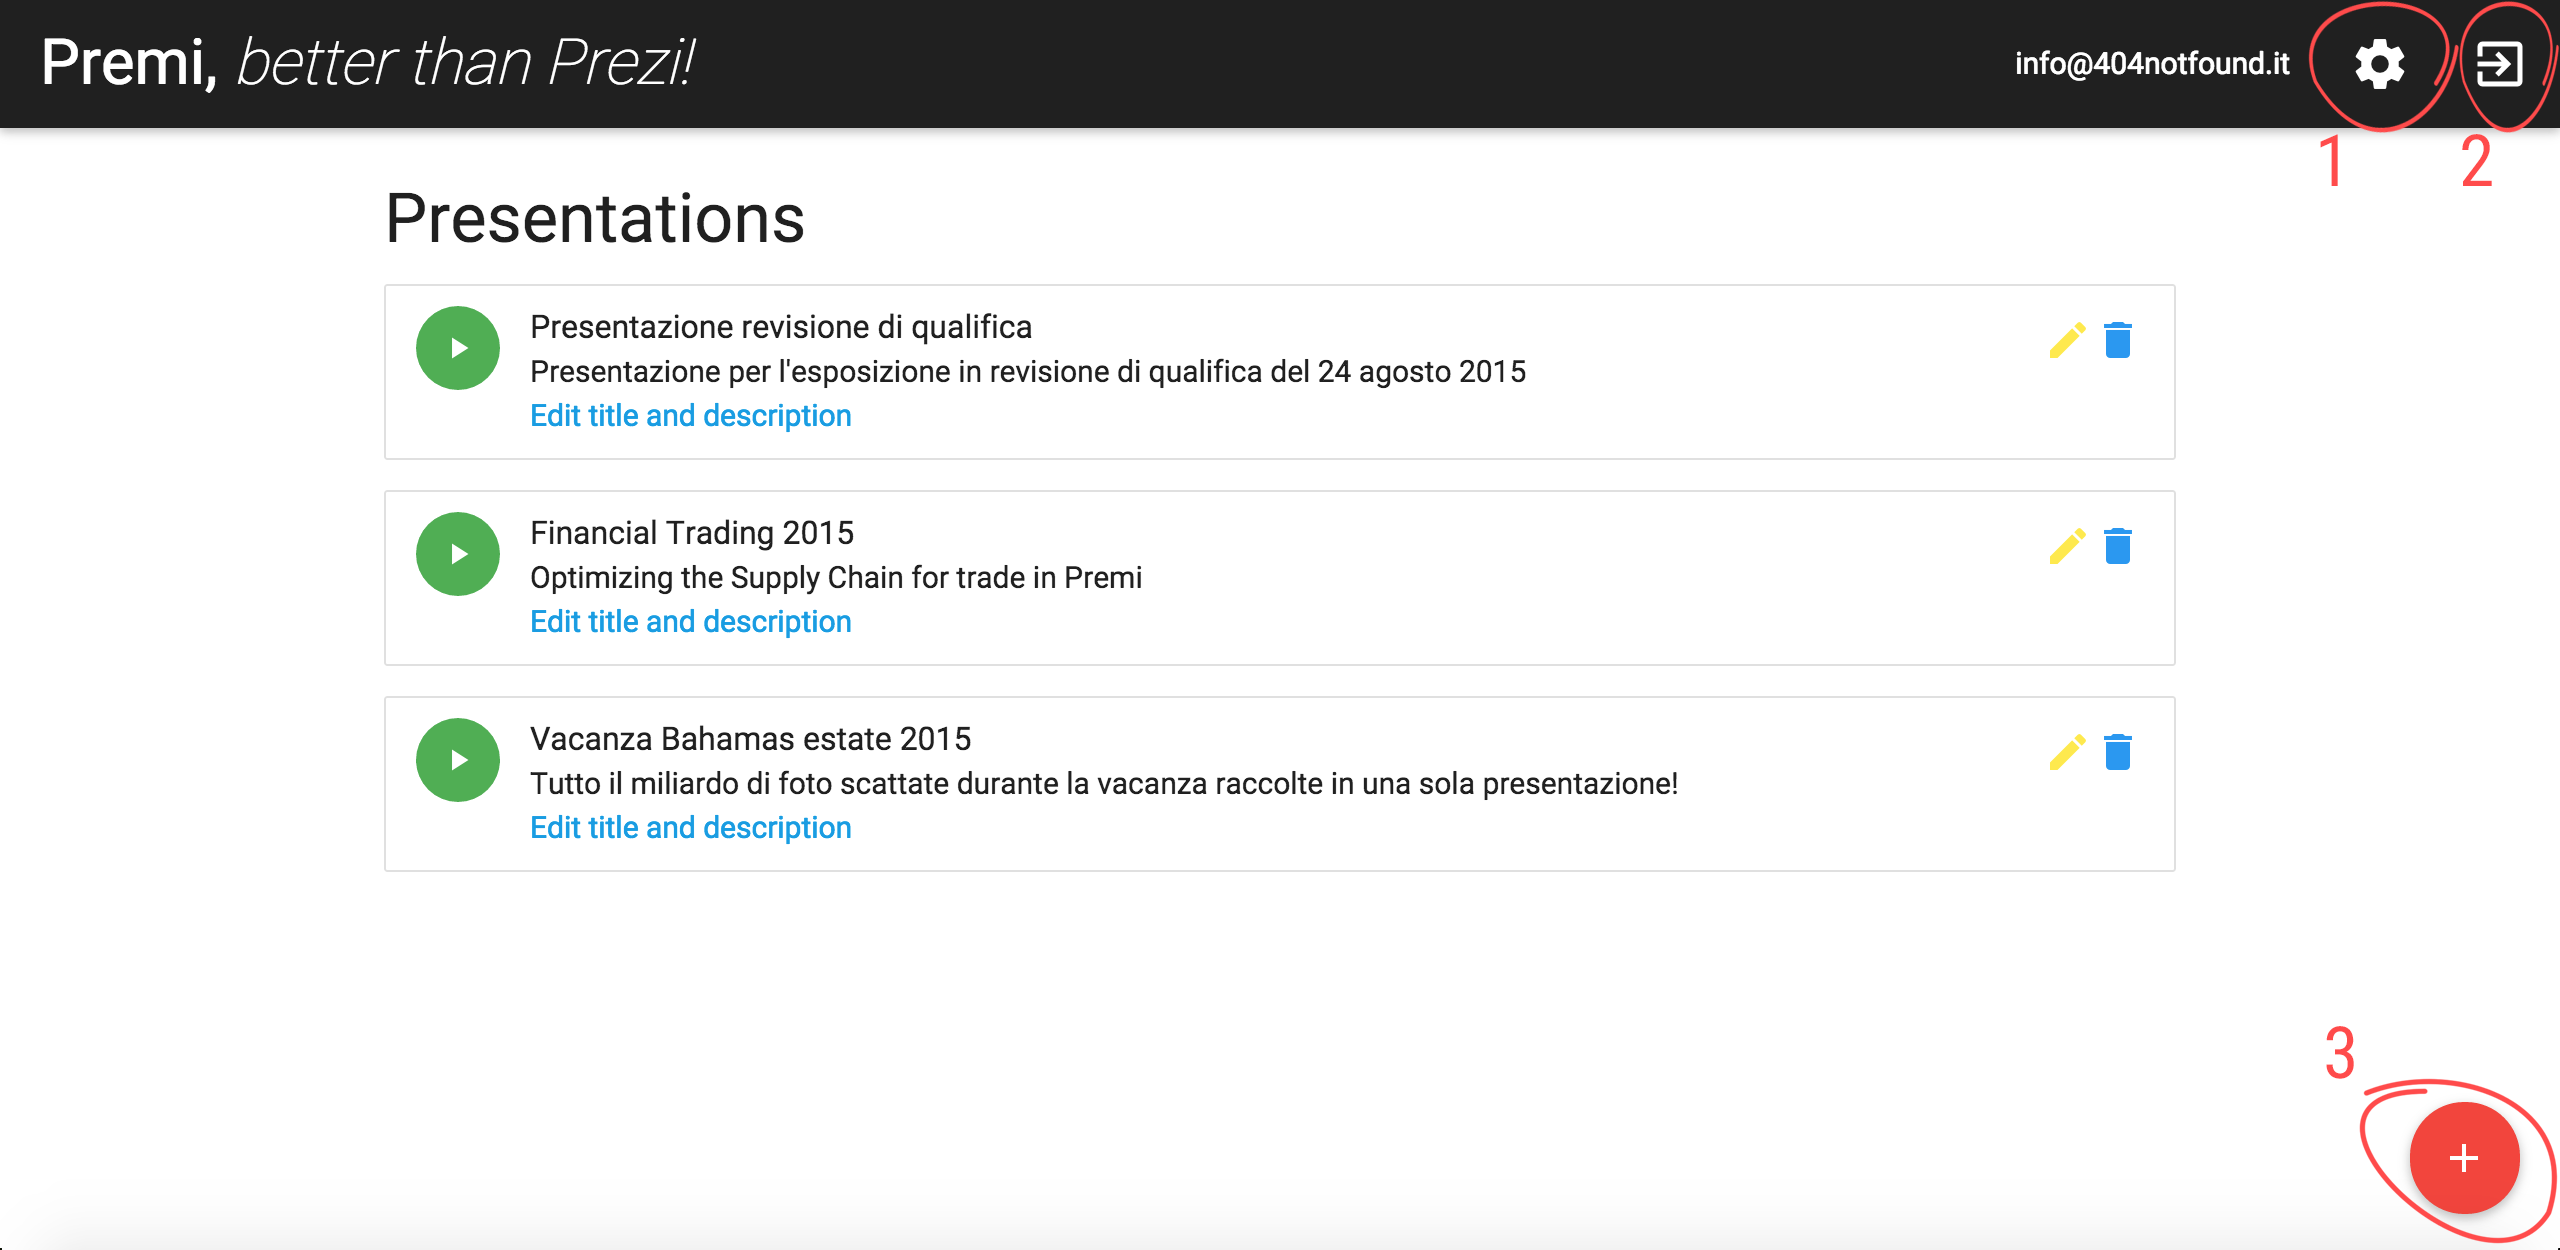
\includegraphics[scale=0.35]{img/dashboard_guide.png}
\caption{Pannello di controllo utente.}
\end{center}
\end{figure}
Comandi:
\begin{enumerate}
\item Permette la modifica dei dati dell'account.
\item Consente all'utente di disconnettersi dal sistema.
\item Permette la creazione di una nuova presentazione.
\end{enumerate}

\subsection{Creare una nuova presentazione}
Come creare una nuova presentazione.

\subsection{Editor}
\subsubsection{Aggiunta frame}
\subsubsection{Aggiunta elemento shape}
\subsubsection{Aggiunta testo}
\subsubsection{Modifica degli elementi}
\subsubsection{Creazione percorso presentativo}
\subsubsection{...........}

\subsection{Gestione presentazioni}
\subsubsection{Eliminazione}
\subsubsection{Modifica}

\subsection{Esportazione}
\subsubsection{Formato 1 (portable?)}
Spiegare anche come eventualmente visualizzare la presentazione in caso di formato portable.
\subsubsection{Formato 2 (poster?)}

\subsection{Avvio di una presentazione}
\subsubsection{Sessione locale}
\subsubsection{Sessione remota}

\subsection{Condivisione di una presentazione}

\subsection{Gestione dati account}

\subsection{Errori e loro cause}

